\documentclass[a4paper,12pt]{scrartcl}
\usepackage[top=2.5cm, bottom=2.5cm, left=1.5cm, right=1.5cm]{geometry}
\usepackage{caption}
%%%%%%%%%%%%%%%%%%%%%%%%%%%%%%%%%%%%%%%%%%%%%%%%%%%%%%%%%%%%%%%%%%%%%%
\usepackage[english]{babel}
\usepackage[utf8]{inputenc}
%\usepackage{epsfig}
%\usepackage{graphicx}
\usepackage{amsmath}
\usepackage{amssymb}
\usepackage{authblk}
%% \usepackage{natbib,twoopt,ifthen}
%\usepackage{aas_macros}
\RequirePackage[colorlinks,breaklinks]{hyperref}  
\hypersetup{linkcolor=blue,citecolor=blue,filecolor=black,urlcolor=blue} 
% write ``draft'' across the pages
\usepackage{draftwatermark}
\SetWatermarkScale{5}
\SetWatermarkLightness{0.90}
\newcommand{\FixMe}[1]{{\bf \large #1}}
\newcommand{\ClName}[1]{{\bf #1}}
\newcommand{\RoutineName}[1]{\texttt{#1}}
\def\arcsec{\hbox{$^{\prime\prime}$}}
%\addmargin{-0.5cm}{-0.5cm}
\providecommand{\eprint}[1]{\href{http://arxiv.org/abs/#1}{#1}}

% KOMA script complains loudly 
% if we use the old font selection macros.
\def\bf{\normalfont\bfseries}
\def\rm{\normalfont \rmfamily}

%%%%%%%%%%%%%%%%%%%%%%%%%%%%%%%%%%%%%%%%%%%%%%%%%%%%%%%%%%%%%%%%%%%%%%
\title{Documentation of the astrometry component of the jointcal package}
%\subtitle{(V0)}
\author{Pierre Astier}
\affil{LPNHE/IN2P3/CNRS (Paris)}


%%%%%%%%%%%%%%%%%%%%%%%%%%%%%%%%%%%%%%%%%%%%%%%%%%%%%%%%%%%%%%%%%%%%%%
\begin{document}

\maketitle

\abstract{The jointcal package aims at optimizing simultaneously
  the WCS's of a set of astronomical images of the same field. This
  approach produces in principle, and often as well in practice, WCS's
  which are more precise than when fitted independently. This is
  especially true when the images are deeper than the astrometric
  reference catalogs. In the ``Astromatic'' software suite, this
  simultaneous astrometry functionality is fulfilled by ``SCAMP''. The
  code we describe here has similar aims, but follows a slightly
  different route. It is meant to be used within the LSST software
  stack framework. }



\tableofcontents

\section{Introduction}
With deep astronomical images, it is extremely common that
the relative astrometry between images is considerably more precise
than the accuracy of external catalogs, where ``more precise'' can be as large
as two orders of magnitude. For applications where the
quality of relative astrometry is important or vital, it is important
to rely on some sort of simultaneous astrometry solution, if possible
optimal in a statistical sense. 

This package performs a least-square fit to a set of images.
Since it aims at statistical optimality, we maximize 
the likelihood of the measurements with respect to all 
unknown parameters required to describe the data.
These parameters consists mostly in two sets: the position
(on the sky) of the objects in common, and the mapping
of each image to the sky. To these obvious parameters,
one can add proper motions (where applicable), and 
parameters describing the differential effect of atmospheric refraction
on the position of objects. It is clear that one cannot
fit simultaneously the position on the sky and the mappings
from CCD coordinates to the sky, without extra constraints:
the ``sky'' coordinate system is then undefined, and one needs
reference positions in order to fully define this frame.
So far, we have used the USNO (A 2.0) catalog for this purpose.


SCAMP\footnote{see \href{http://www.astromatic.net/software/scamp}{http://www.astromatic.net/software/scamp}} is the reference package for simultaneous astrometry in
astronomy, at least for relative alignment of wide-field images prior
to stacking. Regarding optimization, SCAMP follows a somehow different
route from ours: it does not optimize over the position of common
objects but rather minimizes the distance between pairs of transformed
measurements of the same object. This approach is not a maximum
likelihood optimization, and hence is likely sub-optimal statistics
wise. We do not know how sub-optimal it is, but the main drawback of
SCAMP in the context of LSST is the fact that it is a program and not
a library, and hence not flexible regarding formats of images and
catalogs.  But since SCAMP has been used for almost a decade in
production by various teams, the quality checking tools it provides
should likely be reproduced in the context of our package. We provide
residual ntuples and hope that the first serious users will contribute
plotting tools.

The code is heavily biased towards astrometry. One related problem,
important in some of the target applications, is relative {\it
  photometry}.  We have not provided yet the determination of relative
flux scales between images but we plan to do so. The principles are
similar to relative astrometry, but considerably simpler. The main reason
to integrate it to the present package is that loading the input catalogs
takes a large amount of time and so, solving for the relative photometry
once they are in memory looks like a good idea.


The plan of this note goes as follows: we first sketch the algorithm
(\S \ref{sec:algo}). We then describe the first step, i.e. how we
associate the measurements of the same objects in different exposures (\S \ref{sec:assoc}). We provide our least-squares formulation in \S~\ref{sec:ls},
and describe the how we evaluate the derivatives with respect to the parameters.


\section{Algorithm flow \label{sec:algo}}
The algorithm assumes that the input images are equipped with a WCS
accurate to $\sim 1\arcsec$. Currently, the code interprets properly
the SIP WCS's (relying on the IO's from afw), with or without
distortions. The code might handle transparently the ``PV'' encoding
of distortions (used in SCAMP and Swarp), but lacks the 
IO's required to use this format.
Note that in both instances, the WCS boils down to a polynomial 2D
transform from CCD space to a tangent plane, followed by a gnomonic
de-projection to the celestial sphere.  The difference between formats
lies into the encoding of the polynomial, but they map exactly
the same space of distortion functions. 


The algorithm can be roughly split into these successive steps:
\begin{enumerate}
\item load the input catalogs and 'rough' WCS's (the selection
of objects is left to the user)
\item Associate these catalogs, i.e. associate the detections of the
same object in the image set. one can also associate
these ensemble of detections with an external catalog (USNO in practise).
\item Actually fit what should be fitted, with outlier clipping.
\item Output results.
\end{enumerate}


\section{Association of the input catalogs \label{sec:assoc}}
In the LSST stack framework, the reduced input images are called
``Calexp''. Each of those typically holds the data from 1 CCD
and exposure, and associate the ``reduction'' products, typically
a variance map, a catalog and a WCS obtained by matching the catalog to
some external reference. The data from a {\it Calexp} we need for further
processing is stored into a \ClName{CcdImage} object. It basically
stores informations derived from the image FITS header, from the WCS,
and from the image catalog.

\begin{figure}[ht]
\centering
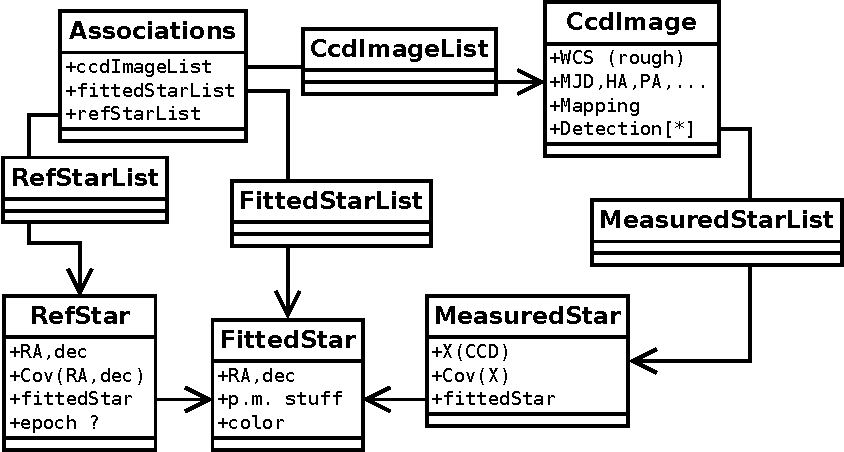
\includegraphics[width=0.8\textwidth]{AssocClasses}
\captionsetup{margin={0.07\textwidth,0.07\textwidth}}% only for this figure
\caption{Chart of class relations which implement the associations
between input catalogs. One \ClName{FittedStar} usually has several
\ClName{MeasuredStar} pointing to it, and each \ClName{RefStar} points 
to exactly one \ClName{FittedStar}. Most \ClName{FittedStar's} have no \ClName{RefStar}.
\label{fig:AssocClasses}
}
\end{figure}


The \ClName{Associations} class holds the list of input
\ClName{CcdImage's} and connects together the measurements of the same
object. The input measurements are called \ClName{MeasuredStar} and
the common detections are called \ClName{FittedStar}. The objects
collected in an external catalog are called \ClName{RefStar}.
Despite their
names, these classes can represent galaxies as well as stars. The
collections of sush objects are stored into \ClName{MeasuredStarList},
\ClName{RefStarList} 
and \ClName{FittedStarList}, which are container derived from \ClName
{std::list}. The relations between these classes, all implemented in C++,
are displayed in figure \ref{fig:AssocClasses}.


\section{Least squares \label{sec:ls}}
\subsection{Least-squares expression}
The fit consists of minimizing:
\begin{align}
\chi^2 & =  \sum_{\gamma,i}  [M_\gamma(X_{\gamma,i})-P_{\gamma}(F_k) ]^T W_{\gamma,i}  [M_\gamma(X_{\gamma,i})-P_{\gamma}(F_k) ] & \textrm{(meas. terms)} \nonumber \\
         &+\sum_j [P(F_j)-P(R_j)]^T W_j [P(F_j)-P(R_j)] & \textrm{(ref. terms)} \label{eq:chi2}
\end{align}
where the first line iterates on all MeasuredStar ($i$) from all
CcdImage (indexed by $\gamma$), and the second iterates on all RefStar
($j$). In the first terms, the object at position $F_k$ is the one
that was measured at position $X_{\gamma,i}$ in image $\gamma$. 
The association between measurements and objects is 
described in the above paragraph. 

    The measurement terms compare the measurement positions
to objects positions, the reference terms compare object positions 
to reference positions. We need these two sets of terms
because not all objects $F_k$ in the first terms appear
in the second terms: there are plenty of objects in the images
which are not in the reference catalogs, but which constrain the
mappings $M_\gamma$ to transform measured coordinates to the
same positions. 

For the measurement terms (first line), the notations are:
\begin{itemize}
\item $M_\gamma$ is the mapping (for CcdImage $\gamma$) from pixel space to
some tangent plane to the celestial sphere, (defined by $P_\gamma$);
\item $P_\gamma$ is a projector from sidereal coordinate to some tangent plane;
$P_\gamma$ is user-defined.
\item $X_{\gamma,i}$ is the position of MeasuredStar $i$ of CcdImage $\gamma$
in pixel space of this CcdImage;
\item $F_k$ is the (sky) position of the FittedStar corresponding 
to this MeasuredStar. In the data structure, the FittedStar is just pointed to 
by the MeasuredStar see fig. \ref{fig:AssocClasses};
\item $W_{\gamma,i}$ is the measurement weight of $M_\gamma(X_{\gamma,i})$, i.e.
the inverse of the 2$\times$2 covariance matrix.
\end{itemize}

The notations for the reference terms (second line) are:
\begin{itemize}
\item $R_j$ refers to the (sky) position of RefStar $j$
\item $F_j$ refers to the (sky) position of the corresponding
FittedStar (i.e. pointed to by the RefStar, see fig. \ref{fig:AssocClasses})
\item $P$ is some (user-provided) projector;
\item $W_j$ is the weight matrix of the projected position $P(R_j)$. 
\end{itemize}

The expression \ref{eq:chi2} above depends on two sets of parameters:
the parameters defining the mappings $M$ and the positions $F_k$.
For a practical problem, this amounts to a very large number of parameters,
which becomes tractable if one remarks that every term in the $\chi2$ 
only addresses a small number of parameters. We exploit this feature 
to compute rapidly the gradient and even the Hessian of the $\chi^2$.

So far, we have not specified how
we model the mappings $M$ nor how we choose the various projectors 
that appear in expression \ref{eq:chi2}. The code has been written
to allow the final user to provide its own version of both the model
for mappings and the projection scheme. We however provide some 
implementations for both aspects that we discuss in the next two sections.

\subsection{The distortion model}
The routines in the \ClName{AstrometryFit} class do not really evaluate
the derivatives of the mappings, but rather defer those to other classes.
The main reason for this separation is that one could conceive
different ways to model the mappings from pixel coordinates to
the tangent plane, and the actual model should be abstract
in the routines accumulating gradient and Jacobian. The class
\ClName{AstrometryModel} is an abstract class aiming at
connecting generically the fitting routines to actual models.
We have so far coded two of these models:
\begin{itemize} 
\item \ClName{SimplePolyModel} implements 
one polynomial mapping per input \ClName{CcdImage} (i.e Calexp).
\item \ClName{ConstrainedPolyModel} implements a model
where the mapping for each CcdImage is a composition of a polynomial
for each CCD and a polynomial for each exposure. For one of the exposures,
the mapping should be fixed or the model is degenerate.
\end{itemize}
For example, if one fits 10 exposures from a 36-CCD camera,
there will be $10\times 36$ polynomials to fit with the first model, and
$10+36$ with the second model. The  \ClName{ConstrainedPolyModel}
assumes that the focal plane of the instrument does not change
across the data set. We could consider coding a model 
made from one \ClName{ConstrainedPolyModel} per set of images
for which the instrument can be considered as geometrically stable.
This is similar to how Scamp models the distortions.

In both of these models, we have used standard polynomials in 2
dimensions rather than an orthogonal set (e.g. Legendre, Laguerre,
...)  because regular polynomials are easy to compose (i.e. one can
easily compute the coefficients of P(Q(X)) ), and they map exactly the
same space as the common orthogonal sets. We have taken care of
``normalizing'' the input coordinates (roughly map the range of fitted
data over the $[-1,1]$ interval), in order to alleviate the well-know
numerical issues associated to fitting of polynomials.

\subsection{Choice of projectors}
In the least squares expression \ref{eq:chi2}, the residuals of the
measurement terms read:
$$
R_{\gamma i} = M_\gamma(X_{\gamma,i})-P_{\gamma}(F_j)
$$
If the coordinates $F_j$ are sidereal coordinates,
the projector $P_\gamma$ determine the meaning of
the mapping $M_\gamma$. If one is aiming at producing
WCS's for the image, it seems wise to choose for
$P_\gamma$ the projection used foe the envisioned WCS,
so that the mapping $M_\gamma$ just describes the 
transformation from pixel space to the projection plane.
For a SIP WCS, one will then naturally choose a gnomonic projector,
so that $M_\gamma$ can eventually be split into the ``CD'' matrix 
and the SIP-specific higher order distortion terms (see \S \ref{sec:sip-wcs}
for a brief introduction to WCS concepts).

So, the choice of the projectors involved in the fit
are naturally left to the user. This is done via a
virtual class \ClName{ProjectionHandler}, an instance
of which has to be provided to the \ClName{AstrometryFit} constructor.
There are obviously ready-to-use \ClName{ProjectionHandler} implementations
which should suit essentially any need. For the standard astrometric
fit aiming at setting WCS's, we provide the \ClName{OneTPPerShoot}
derived class, which implements a common projection point
for all chips of the same exposure. It is fairly easy to implement
derived classes with other policies.

The choice of the projector appearing in the reference terms of
\ref{eq:chi2} is not left to the user because we could not find a good
reason to provide this flexibility, and we have implemented a gnomonic
projection. We use a projector there so that the comparison of
positions is done using an Euclidean metric.


\subsection{Proper motions and atmospheric refraction}
The expression \ref{eq:chi2} above depends on two sets of parameters:
the parameters defining the mappings and the positions $F_k$. This expression
hides two details implemented in the code: accounting for proper
motions and differential effects of atmospheric refraction.

Proper motions can be accounted for to predict the expected positions
of objects and even be considered as fit parameters. At the moment we
neither have code to detect that some (presumably stellar) object is
moving, nor code to ingest proper motions from some external catalog.
Each \ClName{FittedStar} has a flag that says whether it is affected
by a proper motion and the proper motion parameters can all be fitted
or not (see \S \ref{sec:indices_whattofit}).

The code allows to account for differential chromatic effects of 
atmospheric refraction, i.e. the fact that objects positions in the image
plane are shifted by atmospheric refraction in a way that depends on 
their color. The shift reads:
\begin{equation}
\delta X = k_b(c-c_0)\hat{n} \label{eq:refrac_corr}
\end{equation}
where $k_b$ is a fit parameter (one per band $b$), $c$ is the color of
the object in hand, $c_0$ is the average color, and $\hat{n}$ is the
direction of the displacement in the tangent plane (i.e. a normalized
vector along the parallactic direction, computed once for all for each
Calexp).  We have not accounted for pressure variations because they
are usually small, but it would not be difficult. The code accounts
for color-driven differential effects within a given band, but ignores
the differences across bands, would one attempt to fit images from
different bands at the same time. Differences in recorded positions
across bands will be accounted for in the fitted mappings. It is
important to do so because we are fitting WCS's, and we want the fitted
mappings to reflect at best the effects affecting measured
positions. Since the color correction \ref{eq:refrac_corr} is not
accounted for when using WCS's to transform measured position, we have
made this correction zero on average. As for proper motions, fitting
or not these refraction-induced differential position shifts is left
to the user (see \S \ref{sec:indices_whattofit}).

\subsection{Minimization approach}
The expression \ref{eq:chi2} depends on two sets of parameters: the parameters
defining the mappings $M_\gamma(X) \equiv = M_\gamma(\eta_\gamma,X)$,
and the positions $F_k$. There are indeed extra parameter sets and what 
is described here applies as well to those.

We call $\theta$ the vector that gathers
all parameters. For a practical problem its size
can easily reach $10^5$. But the matrix 
$d^2 \chi^2/d \theta^2$ is very sparse, because
there are no terms connecting $F_i$ and $F_j$ if $i \neq j$, and
depending on how the mappings are parametrized, a set of $\eta_\gamma$
parameters could be connected (in the second derivative matrix) 
to only a small set of $F_j$'s. So, it is tempting to search for the 
$\chi^2$ minimum using methods involving the second derivative matrix, 
if we take advantage of its sparseness.

Let us rewrite the $\chi^2$ (expression~\ref{eq:chi2}) as:
\begin{align}
\chi^2 & =  \sum_{\gamma,i}  {R^m_{\gamma i}}^T W_{\gamma,i}  R^m_{\gamma i} \nonumber \\
         & +\sum_j {R^r_{j}}^T W_{j}  R^r_{j} \label{eq:grad_chi2}
\end{align}
where the meaning of the $R$ vectors is easily derived by comparing to
\ref{eq:chi2} (from which we borrow the notations):
\begin{align}
R^m_{\gamma i}  &= M_\gamma(X_{\gamma,i})-P_{\gamma}(F_k) \\
R^r_{j} &= [P(F_j)-P(R_j)]  \label{eq:ref_res}
\end{align}
We want to find the point where $d \chi^2/d \theta = 0$,
where $\theta$ of (size $N_p$) denotes the vector of parameters. We have
\begin{align}
\frac{1}{2} \frac{d \chi^2}{d \theta} & =  \sum_{\gamma,i}  {R^m_{\gamma i}}^T W_{\gamma,i}  H^m_{\gamma i} \nonumber \\
         & +\sum_j {R^r_{j}}^T W_{j}  H^r_{j} \label{eq:gradient}
\end{align}
where the H matrices are $2 \times N_p$ in size and read:
\begin{align}
 H^m_{\gamma i} & = \frac{d {R^m_{\gamma i}}}{ d \theta} \\
  H^r_{j}     & = \frac{d {R^r_{j}}}{ d \theta}
\end{align}
The matrix $W_{\gamma,i}$ is obtained by transporting the measurement
errors through the fitted mapping. This introduces an extra dependency of the
$\chi^2$ on the parameters, that we have decided not to track in the derivatives, because
these errors mostly depend on the mapping scaling, which is very well
determined from the beginning. However, small changes of scaling can
lead to the $\chi^2$ increasing between iterations. This is why we
provide the \ClName{AstrometryModel::freezeErrorScales} which allows
one to uses for there on the {\it current} state of the model to 
propagate errors, even if mappings are updated. $d R^m_{\gamma i}/d \theta$
has two non-zero blocks: the derivatives with respect to the parameters of the $M_\gamma$
mapping
(which are delivered by the Gtransfo-derived class that implements the
fitted mapping, namely by the \ClName{Gtransfo::paramDerivatives} routine); and the derivative with respect to the $F_k$ position which reads $d P_\gamma(F_k)/d F_k$ (delivered as well by the class that implements the projector, via the \ClName{Gtransfo::computeDerivative} routine).

Regarding reference terms, the matrix $W_j$ should be derived from
the reference catalog position uncertainty matrix $V_0$ (typically
delivered for ($\alpha,\delta$) coordinates):
\begin{equation*}
W_j = (P'^T V_0 P')^{-1}
\end{equation*}
where $P'$ is the derivative of the projector. The inverse of $W_j$ is
in practice obtained using the routine
\ClName{Gtransfo::transformPosAndErrors} which is attached to the
projector. The derivative of the reference residual $R^r_{j}$ with respect to
the \ClName{FittedStar} position $F_j$ (see eq. \ref{eq:ref_res}),
is just the $2\times 2$ matrix of the derivative
$P'$ of the projector $P$, which we compute using \ClName{Gtransfo::computeDerivative}.


If one is ready to evaluate the second derivative matrix of the
$\chi^2$, the standard method to zero the gradient
is to Taylor expand it:
$$
\frac{d \chi^2}{d \theta}(\theta_0+\delta\theta) = \frac{d \chi^2}{d \theta}(\theta_0) + \frac{d^2 \chi^2}{d \theta^2}(\theta_0)\delta\theta + O(\delta\theta^2)
$$  
and solve for the offset that zeroes it to first order:
\begin{equation}
\delta\theta =  - \left[ \frac{d^2 \chi^2}{d \theta^2}(\theta_0) \right]^{-1}  \frac{d \chi^2}{d \theta}(\theta_0) \label{eq:step_definition}
\end{equation}
At this stage, if the problem is non-linear (more precisely, if the
second derivative varies rapidly) it is wise to consider a line
search, i.e. to minimize $\chi^2(\theta_0 + \lambda\times
\delta\theta)$ over $\lambda$.

We write the second derivative of our $\chi^2$ (or Hessian) as:
\begin{align}
\frac{1}{2} \frac{d^2 \chi^2}{d \theta^2} & =  \sum_{\gamma,i}  {H^m_{\gamma i}}^T W_{\gamma,i}  H^m_{\gamma i} \nonumber \\
         & +\sum_j {H^r_{j}}^T W_{j}  H^r_{j} \label{eq:def_hessian}
\end{align}
where we have neglected the second derivatives of the $R$
vectors. This is both simple and handy, because this second derivative
is then by construction positive-definite and hence the parameter
offsets (defined in \ref{eq:step_definition}) can be evaluated using
the (fast) Cholesky factorization. This indicates that, if possible,
mappings $M_\gamma(\eta_\gamma,X)$ linear with respect to their
parameter $\eta_\gamma$, for example polynomials, are to be favored.

Since the matrices $W_{\gamma,i}$ are positive-definite, they have
square roots (e.g. the Cholesky square root) and can be written as:
$W_{\gamma,i} = \alpha^T_{\gamma i} \alpha_{\gamma i}$. Defining
$K^m_{\gamma i} = \alpha_{\gamma i} H^m_{\gamma i}$, the Hessian
expression becomes
\begin{align}
\frac{1}{2} \frac{d^2 \chi^2}{d \theta^2} & =  \sum_{\gamma,i}  {K^m_{\gamma i}}^T K^m_{\gamma i} +\sum_j {K^r_{j}} K^r_{j} %\label{eq:def_hessian}
\end{align}
The sums present in this expression can be performed using
matrix algebra. We concatenate all the $K$ matrices into a big
matrix, called the Jacobian matrix:
$$
J \equiv \left[\{K^m_{\gamma i}, \forall \gamma, i\}, \{ K^r_{j}, \forall j\} \right]
$$
and we then simply have
$$
\frac{1}{2} \frac{d^2 \chi^2}{d \theta^2} = J^T J
$$
In the code, we take advantage of the fact that each term of the
$\chi^2$ only depends on a small number of parameters. The data
stuctures allow us to rapidly collect the indices of these parameters,
and we evaluate in fact the $H$ matrices for these indices only.

The computation of the Jacobian and the gradient is performed in
the \ClName{AstrometryFit} class. The methods
\RoutineName{AstrometryFit::leastSquareDerivativesMeasurement} and \\
\RoutineName{AstrometryFit::leastSquareDerivativesReference} evaluate the contributions to
the Jacobian and gradient of the $\chi^2$ from the measurement terms
and the references terms respectively. In these routines, the Jacobian
is represented as a list of triplets $(i,j,J_{ij})$ describing its
elements. This list is then transformed into a representation of
sparse matrices suitable for algebra, and in particular suitable to
evaluate the product $J^TJ$. Once we have evaluated $H\equiv J^TJ$, we
can solve $HX=-g$ (see eq. \ref{eq:step_definition}, where the Hessian, $H$, is as
defined in \ref{eq:def_hessian}, $X$ is the vector of parameter/fittedStar deltas
we are solving for, and $g$ is the gradient of the $\chi^2$, given in \ref{eq:gradient})
using a Cholesky factorization. For sparse linear
algebra, the Cholmod and Eigen packages provide the required
functionality. It turns out that for practical problems, the
calculation of $J^TJ$ or the factorization are the most CPU intensive
parts of the calculations, and
there is hence not much to be gained in speeding up the calculation of
derivatives. For the factorization, we have tried both Eigen and
Cholmod (via the Eigen interface) and their speeds differ by less
than 10\%.

\subsection{A small note about our choice for linear solvers}
The standard Cholesky decomposition of a matrix H consists in finding
a factor $L$ such that $H = LL^T$, with L triangular (possibly after a
permutation of indices). Both Eigen and Cholmod offer a variant, $H = LDL^T$, 
where D is diagonal and L (still triangular) has 1's on its diagonal. We
have settled for this variant, because it offers improved numerical stability
and allows one, if needed, to add constraints (via Lagrange multipliers)
to the problem. We have also improved the Eigen interface to
Cholmod by exposing to the user the factorization update capability
of Cholmod, which considerably speeds up the outlier removal.
This is done in the CholmodSimplicialLDLT2 class. Using Cholmod has 
a drawback: we need its run-time library. Cholmod is now packaged 
in SuiteSparse, much bigger than what we need. This is why we packaged
the smallest possible subset of SuiteSparse that fulfills our needs 
into jointcal\_cholmod.


%In the basic tests we have performed (with typically $\sim 1000$ calexps),
%factorizing the Hessian requires typically 10s while computing the
%Jacobian and gradient takes of the order of 1s.


\subsection{Indices of fits parameters and Fits of parameter subsets \label{sec:indices_whattofit}}
Since we use vector algebra to represent the fit parameters, we need
some sort of mechanism to associate indices in the vector parameter to
some subset (e.g. the position of an FittedStar) of these parameters.
Furthermore, the implementation we have chosen does not allow
trivially to allocate the actual parameters at successive positions in
memory. The \RoutineName{AstrometryFit::AssignIndices} takes care of
assigning indices to all classes of parameters. For the mappings, the
actual \ClName{AstrometryModel} implementation does this part of the
job. All these indices are used to properly fill the Jacobian and
gradient, and eventually to offset parameters in the
\RoutineName{AstrometryFit::OffsetParams}.

Since the indexing of parameters is done dynamically, it is
straightforward to only fit a subset of parameters. this is why the routine
\RoutineName{AstrometryFit::AssignIndices} takes a string argument that specifies
what is to be fitted.

\section{Fitting the transformations between a set of images}
Some applications require to determine transformations between images
rather than mappings on the sky. For example a simultaneous fit of PSF
photometry for the computation of the light curve a point-like
transient requires mappings between images to transport the common
position in pixel space from some reference image to any other
in the series. The calexp series would typically involve
the CCD from each exposure that covers the region of interest.
The package described here can fit for the needed mappings:
\begin{itemize}
\item in order to remove all reference terms from the $\chi^2$ of eq.~\ref{eq:chi2},
one just avoids to call \RoutineName{Associations::CollectRefStars}.
\item One chooses polynomial mappings for all Calexp 
  but one which will serve as a reference and have a fixed identity mapping.
The distortion model \ClName{SimplePolyModel} allows to do that.
\item Chose identity projectors (the class \ClName{IdentityProjector} does precisely that).
\end{itemize}
So, fitting transformations between image sets can be done with
the provided code. 

\section{Run example}
\begin{verbatim}

        assoc = Associations()

# iterate on the input calexps        
        for dataRef in ref :
            src = dataRef.get("src", immediate=True)
            calexp = dataRef.get("calexp", immediate=True)
            tanwcs = afwImage.TanWcs.cast(calexp.getWcs())
            bbox = calexp.getBBox()
            md = dataRef.get("calexp_md", immediate=True)
            calib = afwImage.Calib(md)
            filt = calexp.getFilter().getName()
# select proper sources            
            newSrc = ss.select(src, calib)

# actually load the data            
            assoc.AddImage(newSrc, tanwcs, md, bbox, filt, calib,
                           dataRef.dataId['visit'], dataRef.dataId['ccd'],
                           dataRef.getButler().mapper.getCameraName(), 
                           astromControl)

# carry out the association        
        matchCut = 3.0
        assoc.AssociateCatalogs(matchCut)
# collect reference objects
        assoc.CollectRefStars(False) # do not project RefStars
# select objects measured at least twice.
        assoc.SelectFittedStars()
# Send back fitted stars on the sky.
        assoc.DeprojectFittedStars() # required for AstrometryFit
# Chose a ProjectionHandler
        sky2TP = OneTPPerShoot(assoc.TheCcdImageList())
# chose a distortion model
        spm = SimplePolyModel(assoc.TheCcdImageList(), sky2TP, True, 0)
# Assemble the whole thing
        fit = AstrometryFit(assoc,spm)
# we are ready to run. Initialize parameters by running "partial fits"
        fit.Minimize("Distortions")
        fit.Minimize("Positions")
# now fit both sets simultaneously.
        fit.Minimize("Distortions Positions")
# output residual tuples
        fit.MakeResTuple("res.list")
\end{verbatim}
  




\appendix
\section{Representation of distortions in SIP WCS's \label{sec:sip-wcs}}
The purpose of the appendix is to provide the minimal introduction
to WCS concepts required to understand the code (and the comments)
when browsing through it. Readers familiar with WCSs can give up here.

WCS's are abstract concepts meant to map data on coordinate systems.
In the astronomical imaging framework, this almost always means
mapping the pixel space into sidereal coordinates, expressed in some
conventional space\footnote{The WCS concepts are broad enough to
  accommodate mapping of planet images, but we will obviously not
  venture into that.}. One key aspect of the WCS ``system'' is that
it proposes some implementation of the mappings in FITS headers, which comes
with software libraries to decode and encode the mappings. The WCS conventions
cover a very broad scope of applications, and wide-field imaging
makes use of a very small subset of those. 

For the mappings used in wide-field imaging, the transformation
from pixel space to sky can be pictured in two steps:
\begin{enumerate}
\item mapping coordinates in pixel space onto a plane.
\item de-projecting this plane to the celestial sphere.
\end{enumerate}
Let us clear up the projection/de-projection step first. There are
plenty of choices possible here, and the differences only matter fir
really large images. The projection used by default in the imaging
community seems to be the gnomonic projection: the intermediate space
is a plane tangent to the celestial sphere and the
plane$\rightarrow$sphere correspondence is obtained by drawing lines
that go through the center of the sphere. In practice there is no need
to know that, because any software dealing with WCS's can pick up the
right FITS keywords and compute the required projection and
de-projection.  For this gnomonic projection, one finds
\verb&CTYPE1='RA---TAN'& and \verb&CTYPE2='DEC--TAN'& in the FITS
header. This projection is often used to generate re-sampled and/or
co-added images and one should keep in mind that, for large images,
the pixels are not exactly iso-area.  One point of convention that
might be useful to keep in mind; is that WCS conventions express
angles in degrees. In the gnomonic projection, offsets in the tangent
plane are expressed in degrees (defined through angles along great
circles at the tangent point), so that the metric in the tangent plane
is ortho-normal), and sidereal angles evaluated on the sky are also
provided in degrees by the standard implementations. A notable
exception is the LSST software stack where, by default,
the angles are provided in radians.

We now come back to the first mapping step, i.e. converting
coordinates measured in pixel units into some intermediate coordinate
system.  The universal WCS convention here is pretty minimal: it
allows for an affine transform, which is in general not sufficient to
map the optical distortions of the imaging system, even after a clever
choice of the projection. Extensions of the WCS convention have been
proposed here, but none is universally understood. The LSST software
stack implements the SIP addition, which consists in applying a 2-d
polynomial transform to the CCD space coordinates, prior to entering
the standard WCS chain (affine transform, then de-projection). In practice,
the SIP ``twisting'' is applied by the LSST software itself 
(in the class \ClName{afw::image::TanWcs}), and 
the ``standard'' part (affine and de-projection, or the reverse transform)
are sub-contracted to the ``libwcs'' code. 

One common complication of the WCS arena is that it was designed
in the FITS framework convention, itself highly fortran-biased
for array indexing, so that the first corner pixel of an image is 
indexed (1,1). The LSST software, and most modern environments use
C-like indexing, i.e. images stars at (0,0), as well as coordinates
in images. The WCS LSST software hides this detail to users, by
offsetting the pixel space coordinates provided and obtained from
the wcs-handling library.

We now detail what is involved in the SIP convention: the SIP
``twisting'' itself is encoded through 4 polynomials of 2 variables,
which encode the direct and reverse transformations. The standard
affine transform is expressed through a $2\times 2$ matrix ($Cd$) and
a reference point $X_{ref}$ (called \verb'CRPIX' in the fits header):
$$
 Y_{TP} = Cd (X_{pix} - X_{ref})
$$
$X_{pix}$ is a point in the CCD
space, and $Y_{TP}$ is its transform in the tangent plane. Obviously,
$X_{pix}$ and $ X_{ref}$ should be expressed in the same frame so that
the transform does not depend this frame choice. We write symbolically
this transform as $ Y_{TP} = L(X_{pix})$
The SIP distortions are defined by a polynomial transformation
in pixel space, that we call $P_A$, for the forward transformation.
By convention, the transform from pixel space to tangent plane then
reads:
$$
 Y_{TP} = L\left( X_{pix} - X_{ref} + P_A( X_{pix} - X_{ref}) \right )
$$
which again does not depend on the frame choice (0-based or 1-based),
provided $X_{pix}$ and $X_{ref}$ are expressed in the same frame.

In jointcal ,the internal representation of SIP WCS's uses three
straight 2d$\rightarrow$2d transformations: the SIP correction, the
affine transformation and the de-projection. Those are just composed
to yield the actual transform, and the two first ones are generic
polynomial transformations. We provide routines to translate the
TanWcs objects into our representation (\RoutineName{ConvertTanWcs})
and back (\RoutineName{GtransfoToTanWcs}). In the latter case, we also
derive the reverse distortion polynomials, which are built if needed
in our representation of SIP WCSs.












\end{document}
%%%%%%%%%%%%%%%%%%%%%%%%%%%%%%%%%%%%%%%%%%%%%%%%%%%%%%%%%%%%%%%%%%%%%%
%%% Local Variables:
%%% mode: latex
%%% eval: (flyspell-mode 1) 
%%% ispell-local-dictionary: "american"
%%% End:
